\documentclass{dasc}

\addbibresource{references.bib}


\title{\uppercase{INSERT PAPER TITLE HERE (NO MORE THAN 80 CHARACTERS)}}

\begin{document}

\author{
	Insert Author’s Name, Company or Affiliation, City, State (if not USA include Country)\\
	Insert Co-Author’s Name, Company or Affiliation, City, State (if not USA include Country)\\
	(If you have multiple authors from the same company, list authors' names first,\\
	followed by company or affiliation, city and state. Do NOT include email addresses here.)
}

\maketitle

\section*{Abstract}

It is not necessary that this abstract be the same as the abstract you previously submitted. This abstract should be a synopsis of your paper. It will generally not be longer than the first column of your paper.

\section*{Do This First!}

Before you do anything else, please print a copy of this file! It contains instructions for producing your paper for the 34th DASC. This file is also a template for creating your paper; you can delete or type over these instructions to help you get started. Finally, the printed version of these instructions will serve as a visual reference of how your finished paper should look.

\section*{Title}

The title of your paper should not exceed 80 characters in length, including spaces. If your title exceeds the 80 character limit, the title will be truncated in signage at the Conference.


\section*{Other Things You Need to Know About Formatting Your Paper}

This section outlines other formatting actions required for 34th DASC publications. 

\subsection*{Length}

Papers should be 8 to 15 pages in length.

\subsection*{Tables}

Table titles should be less than 40 characters with more detailed explanations in the text with a specific reference to the appropriate table (see \cref{tab:example table}).

\begin{table}
\centering
\caption{Sample Table and Table Caption \label{tab:example table}}
\begin{tabular}{llll}
	\toprule
	Sample Description & X & Y & Z \\ \midrule
	Sample Test 1 & 1 & 2 & 3 \\
	Sample Test 1 & 1 & 2 & 3 \\
	Sample Test 1 & 1 & 2 & 3 \\
	\bottomrule	
\end{tabular}
\end{table}

\subsection*{Graphics}

\Cref{fig:example figure} shows an example figure with a caption.

\begin{figure}
\centering
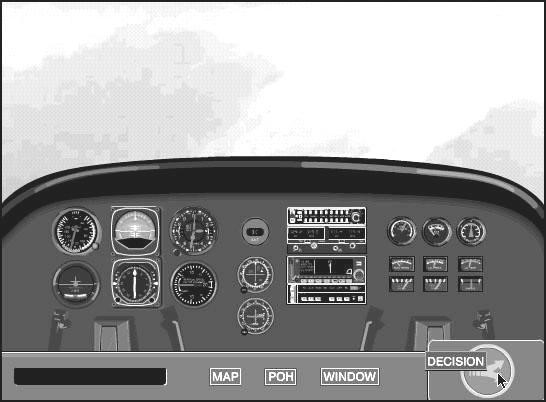
\includegraphics[width=\columnwidth]{figure.jpg}
\caption{Example of a Figure and Caption \label{fig:example figure}}
\end{figure}

\section*{References}

References will be typeset for you using the IEEE biblatex package. Here is an example of a reference \cite{Einstein1935}.

\section*{Acknowledgments}

If an acknowledgment is necessary, include it under the section Acknowledgments.

\section*{Disclaimer}

If a disclaimer is necessary, include it under the section Disclaimer and include the disclaimer immediately after the acknowledgments.

\section*{Submitting Your Final Paper for Review and Approval}

As soon as you have completed the final version of your paper, submit it electronically at: \url{www.dasconline.org}. This must be done no later than August 13, 2015 to ensure adequate time for review and publication.
If you opted for a peer-review of your paper, a draft should be provided to your session chair by June 1, 2015.
Name the file using your abstract number and up to the first five (5) letters of your last name (i.e., for abstract number 115, author Michael L. Johnson would save his file as: 115johns.pdf.) Omit any spaces in your last name when naming your file (i.e., for abstract number 122, author Tom de Jong would save his file as: 122dejon.pdf).
If you cannot submit the paper via \url{www.dasconline.org}, or your paper is more than 25MB, two additional options are available:
\begin{itemize}
	\item Email (if less than 15 MB in size); or
	\item Send a CD, or DVD by postal service to the Publications Editor at the address below, under heading “Additional Documentation Requirements” 
\end{itemize}

The point of this conference is to foster a healthy information exchange among government and industry representatives.  If you upload a paper for publication, then at least one of the authors listed on the paper is expected to attend and present that paper.  IEEE reserves the right to exclude a paper from distribution after the conference (e.g., removal from IEEE Xplore) if the paper is not presented at the conference.  Please register for the conference at \url{www.dasconline.org}.

\section*{IEEE Copyright Form}

All DASC papers are published through IEEE.  Download the 34th DASC official IEEE Copyright Form from \url{www.dasconline.org}. Complete, and sign the form. Submit the form to the Publications Editor, via one of the following options: 
\begin{itemize}
\item Scan to pdf or graphic file (jpg, gif, png, tif) and email
\item Fax
\item Postal service (Please note: Overnight delivery service is recommended; in case their tracking service is required for lost documents).
\end{itemize}

\noindent To:

\noindent Tony Rossetti\\
ALR International\\
3311 Dupree Avenue\\
Orlando, FL 32806-3411\\
\url{pub.editor@dasconline.org}\\
Fax: 888.338.3537 (toll free)\\

All required documents must be received no later than August 13, 2015 to ensure adequate time for review and publication.

Please be aware of any additional release requirements that you may have above and beyond the ones imposed by this conference.  Of particular interest are project sponsor and customer releases.  Many companies also have their own publication release processes that must be satisfied prior to submitting the paper to the 34th DASC.  Remember that it becomes public domain once you upload it.

\printbibliography

\vspace{1cm}
\centering
\emph{\large 34th Digital Avionics Systems Conference\\September 13--17, 2015}

\end{document}